\section{Data}\label{section:data}
\todoyellow{Antager at der er vist et billede med dataen tidligere}
The data provided for this project consists of five three dimensional films of the pancreas of mice, while the pancreas develops over time.
Including time and colour channels, means that the data consists of five dimensions.
The colour channels does not represent the typical RGB, but is the product of different lasers interacting with tissue, and a fluorescent material injected into the mice.
The fluorescent material mainly interacts with the wall of the tubular structure.
In table \ref{tab:data_overview} a overview of the data from a prestudy is shown.

Only the "green" colour channel interacts with the fluorescent material, so the other channels were excluded, reducing the dataset to four dimensions.
The last 20 timesteps of the dataset 3, 4 and 5 the pancreas cells died, and showed no further development.
It was thus discarded.
\begin{table}[h!]
\centering
\begin{tabular}{|l|l|l|l|l|l|l|} \hline
    Dataset & Width & Height & Depth & Timesteps & Colours & mouse id \\ \hline
    1 & 1024 & 1024 & 40 & 159      & 1(3) & 1 \\ \hline
    2 & 1024 & 1024 & 40 & 159      & 1(3) & 1 \\ \hline
    3 & 1024 & 1024 & 27 & 111(131) & 1(3) & 2 \\ \hline
    4 & 1024 & 1024 & 27 & 111(131) & 1(3) & 2 \\ \hline
    5 & 1024 & 1024 & 27 & 111(131) & 1(3) & 2 \\ \hline
\end{tabular}
\caption{Overview of datasets. Original size in the parenthesis, while used
size without parenthesis.}
\label{tab:data_overview}
\end{table}

Only a small part of the data came with labels.
The labels were annotated in a way, so images were only partly labeled, and labels were concentrated around edges of foreground structure and big swathes of background outside of the general structure.
No annotation had been done in the inner of any tubular structure, and only very little foreground was present.


\subsection{Data incoherence} % (fold)
\label{sub:data_incoherence}
In the initial data study, the sums of all images in the datasets where ploted to check for inconsistensies\todoyellow{Ikke stavet rigtigt?}.
This generated the plot shown in Figure~\ref{fig:intensity_densities}.
It can be seen here that dataset 1 and 2 looks very different from dataset 3, 4 and 5.
\begin{figure}[H]
    \centering
    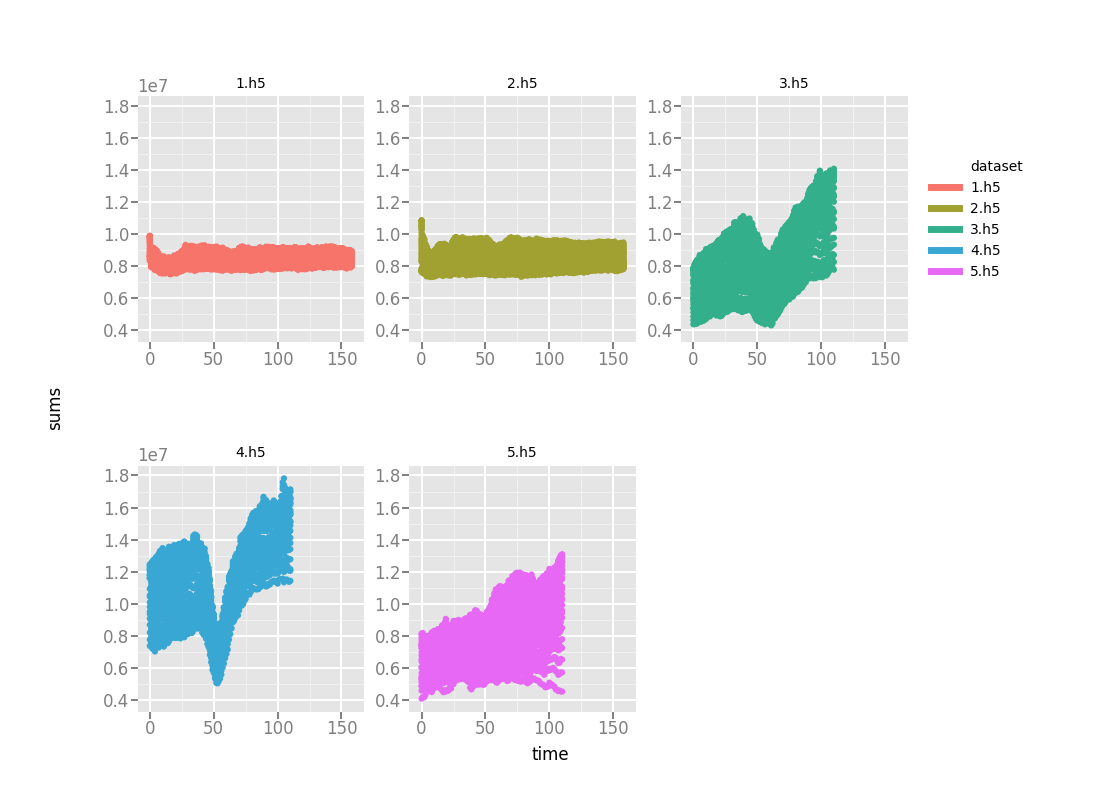
\includegraphics[width = 2.8in]{img/sum_density_t.png}
    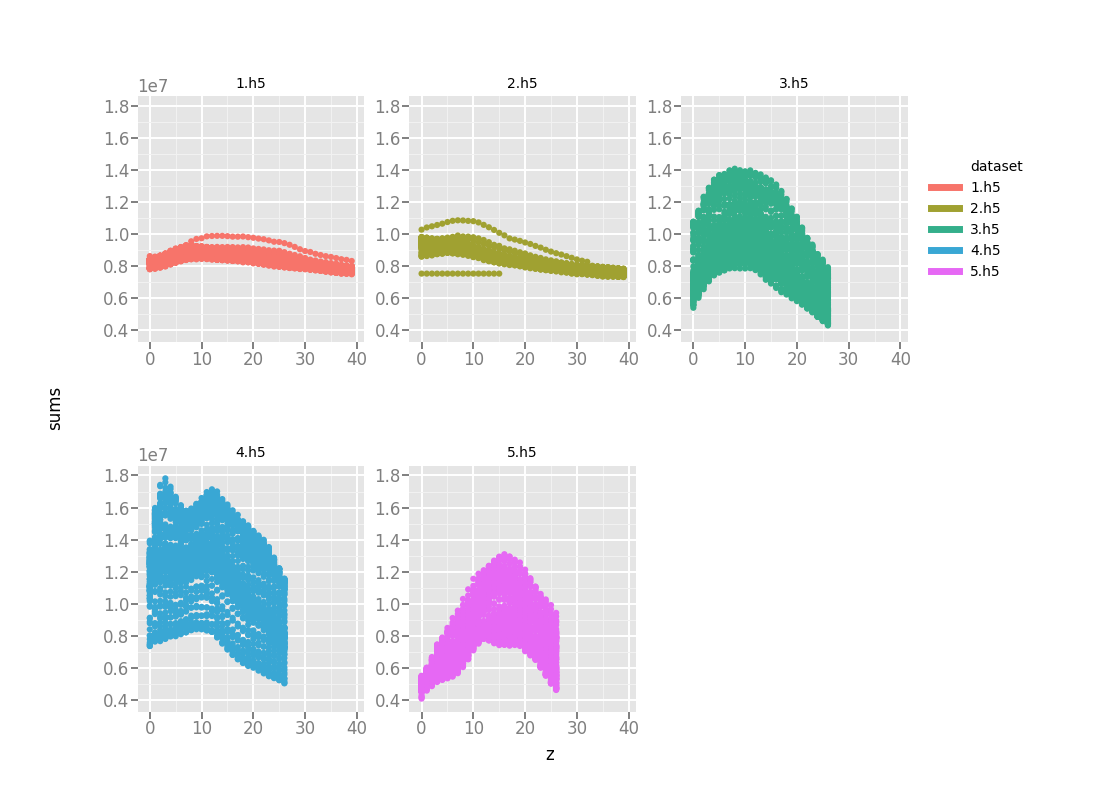
\includegraphics[width = 2.8in]{img/sum_density_z.png}
    \caption{Sum over intensities over axis t and axis z}
    \label{fig:intensity_densities}
\end{figure}

After discussing this with the biology supervisor, we decided to ignore dataset 1 and 2, as they looked preprocessed, and we did not have any idea how and when in the process they had been preprocessed.
% subsection data_incoherence (end)

\subsection{Bad label mappings} % (fold)
\label{sub:bad_label_mapping}
It was discovered that the annotated labels for dataset 3, 4 and 5, did not directly match the image it was paired with.
Because of this and the fact that we wanted to predict the whole structure it was decided to scrap those images and focus on creating new annotations instead of remapping the old labels to the correct image.
% subsection bad_label_mapping (end)

\subsection{New labels} % (fold)
\label{sub:new_labels}
As a result of the bad labels as mentioned in Section~\ref{sub:bad_label_mapping} new labels are required to train a classifier.
These new labels were done by me, and the goal was not to make perfect labels, but rather to make labels good enough to show that the method works.

A previous study of the data had succesfully tried to used clustering of patches, and it was decided that to ease the annotation process, we would preprocess the data with kmeans clustering.
The centroids were retrained on each slice of the image, but the centroid were initialised to be the same as from the previous image.
This way the centroid were almost the same for each image, but would rearrange based on contents of te current image.

\begin{figure}[H]
    \centering
    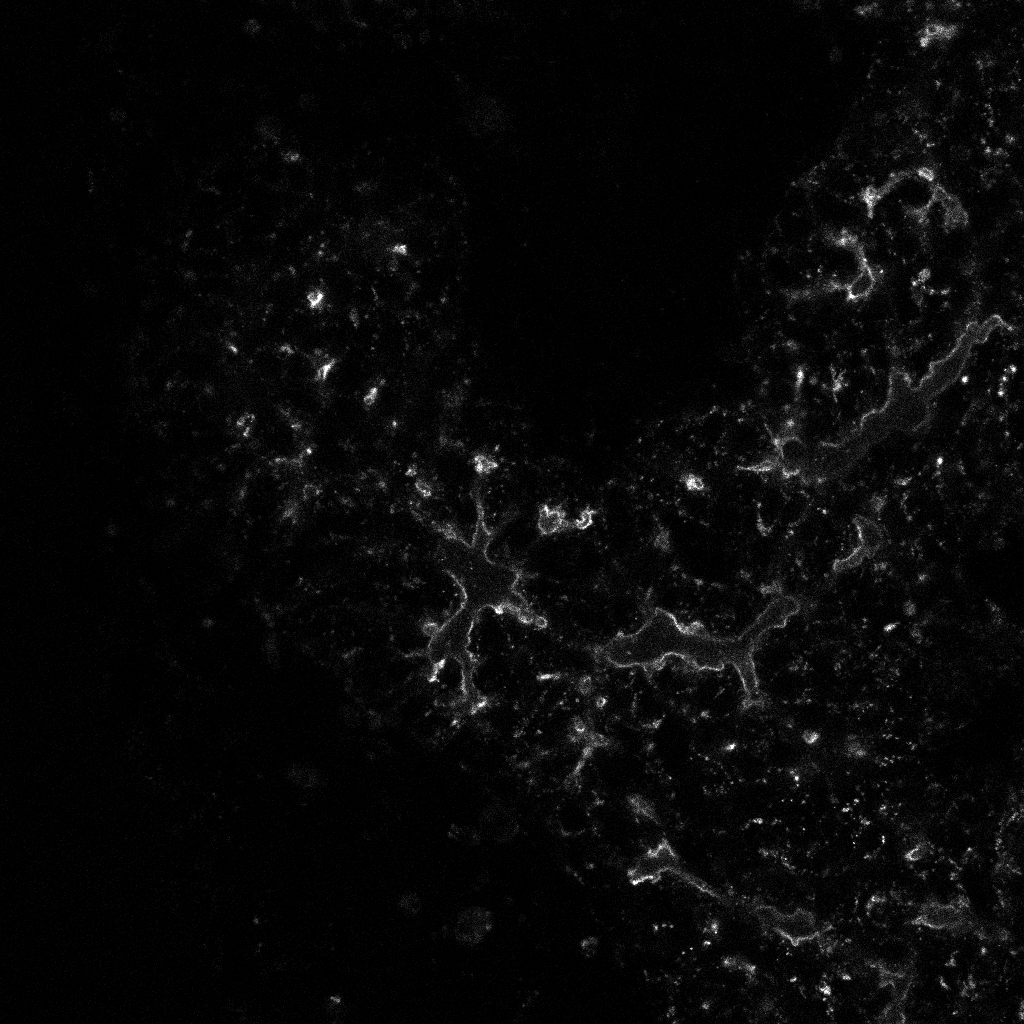
\includegraphics[width=2.8in]{img/3h5022_16.png}
    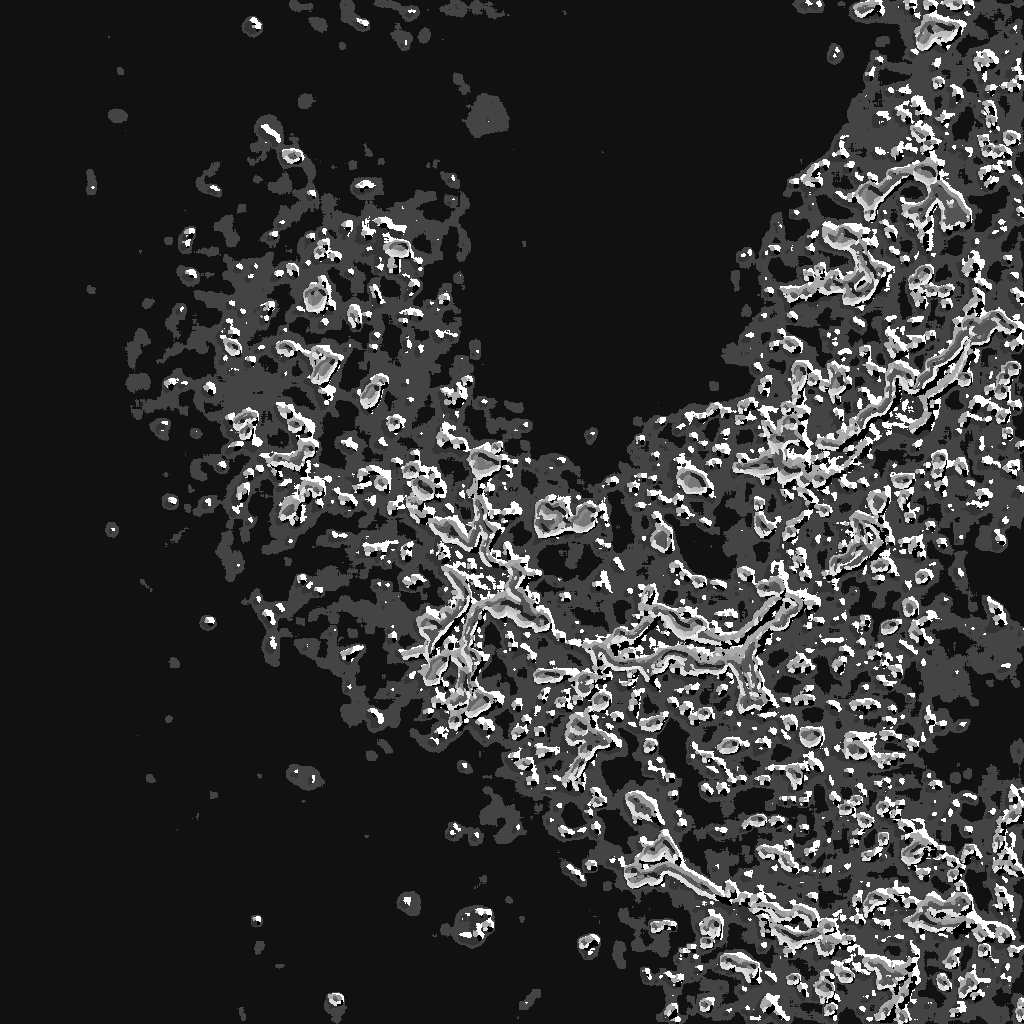
\includegraphics[width=2.8in]{img/3h5022_16_pred.png}
    \caption{An example of the clusters}
    \label{fig:clustering_example}
\end{figure}

\subsubsection{labeling difficulties} % (fold)
\label{ssub:labeling_difficulties}
Even though kmeans helped the annotation process greatly, it was still very hard for someone with little knowledge about the workings of the pancreas, to make great annotations.
As a result of this the most important and difficult areas around the edges of the structure, is not annotated when there is the slightest difficulty doing it.
% subsubsection labeling_difficulties (end)
% subsection new_labels (end)
